
% This LaTeX was auto-generated from MATLAB code.
% To make changes, update the MATLAB code and republish this document.

\documentclass{article}
\usepackage{graphicx}
\usepackage{color}

\sloppy
\definecolor{lightgray}{gray}{0.5}
\setlength{\parindent}{0pt}

\begin{document}

    
    
\subsection*{Contents}

\begin{itemize}
\setlength{\itemsep}{-1ex}
   \item Perform regression [1]
   \item MSE
   \item istogrammi
   \item dagli istogrammi capiamo che la dist
   \item CHIEDERE !!!!!! a\^{} che abbiamo trovato, per trovare la 7esima feature
   \item si fa la combinazione lineare di a\_hat * la riga relativa a un paziente
   \item con tutte le sue features?
   \item the gradient algorithm
   \item istogrammi
   \item steepest descent
   \item istogrammi
\end{itemize}


\subsection*{Perform regression [1]}



\subsection*{MSE}



\subsection*{istogrammi}



\subsection*{dagli istogrammi capiamo che la dist}

\begin{par}
degli errori ? circa una gaussiana? a cosa ? dovuto?
\end{par} \vspace{1em}


\subsection*{CHIEDERE !!!!!! a\^{} che abbiamo trovato, per trovare la 7esima feature}



\subsection*{si fa la combinazione lineare di a\_hat * la riga relativa a un paziente}



\subsection*{con tutte le sue features?}


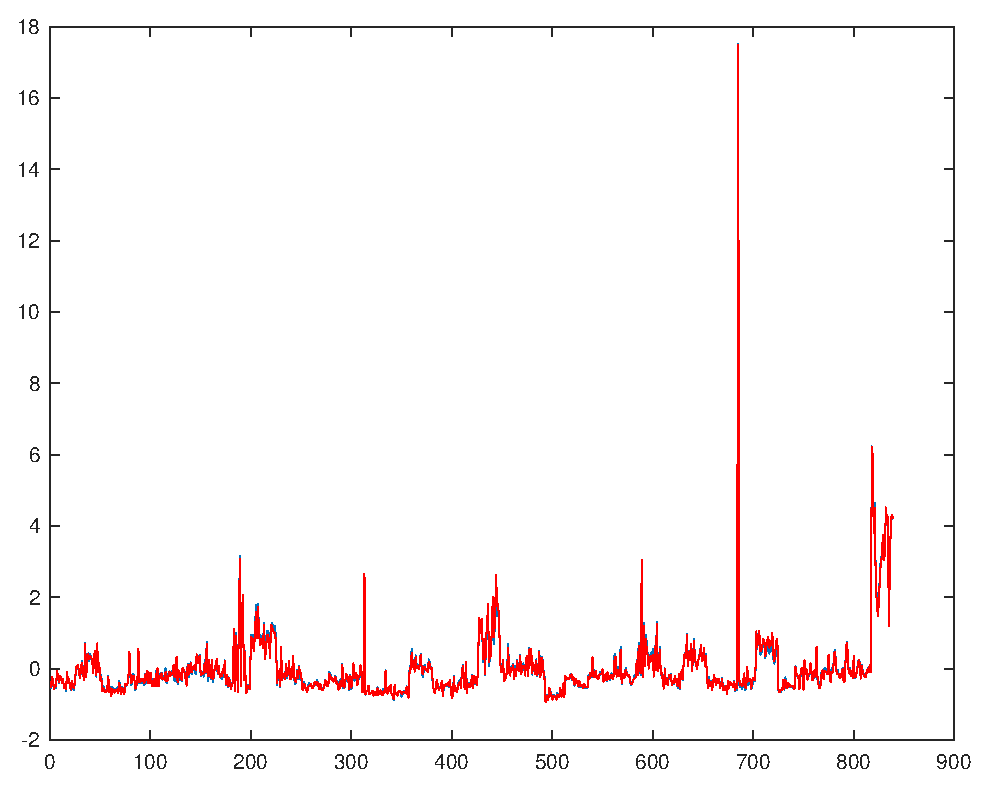
\includegraphics [width=4in]{lab1_01.eps}

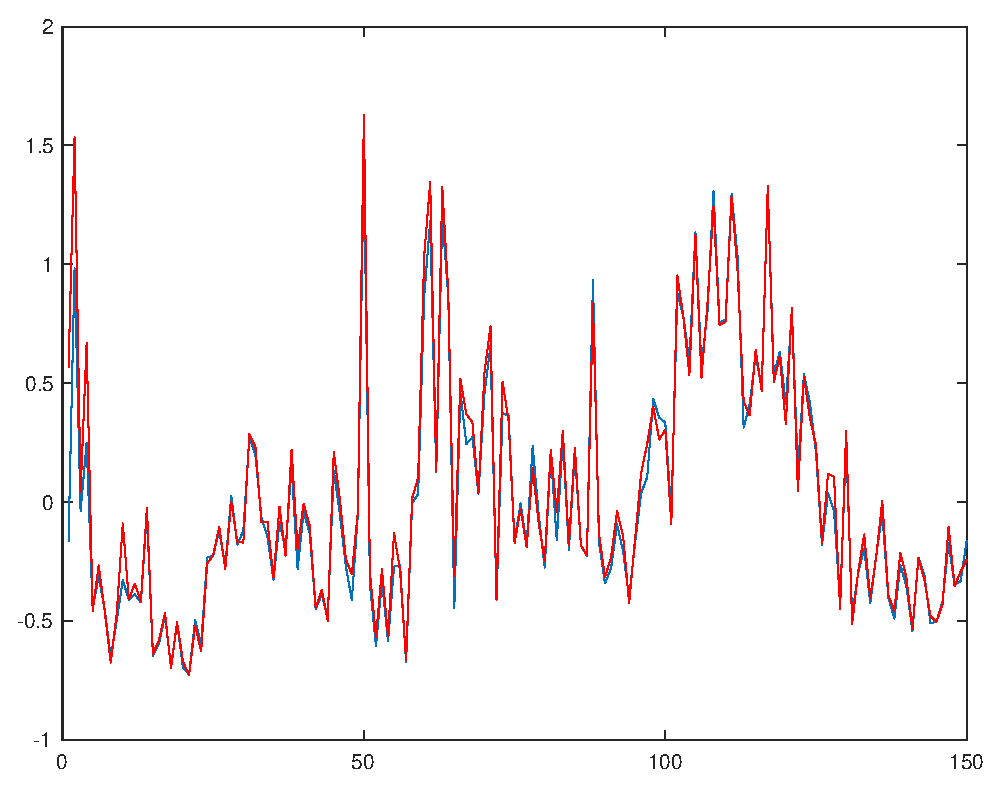
\includegraphics [width=4in]{lab1_02.eps}

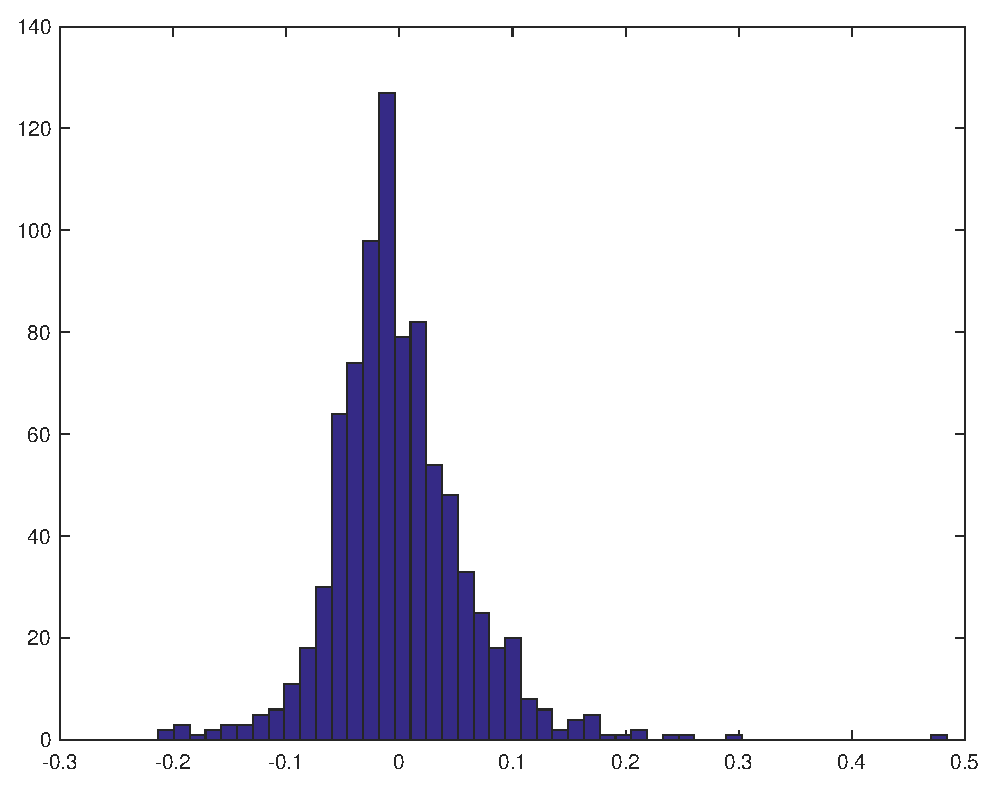
\includegraphics [width=4in]{lab1_03.eps}

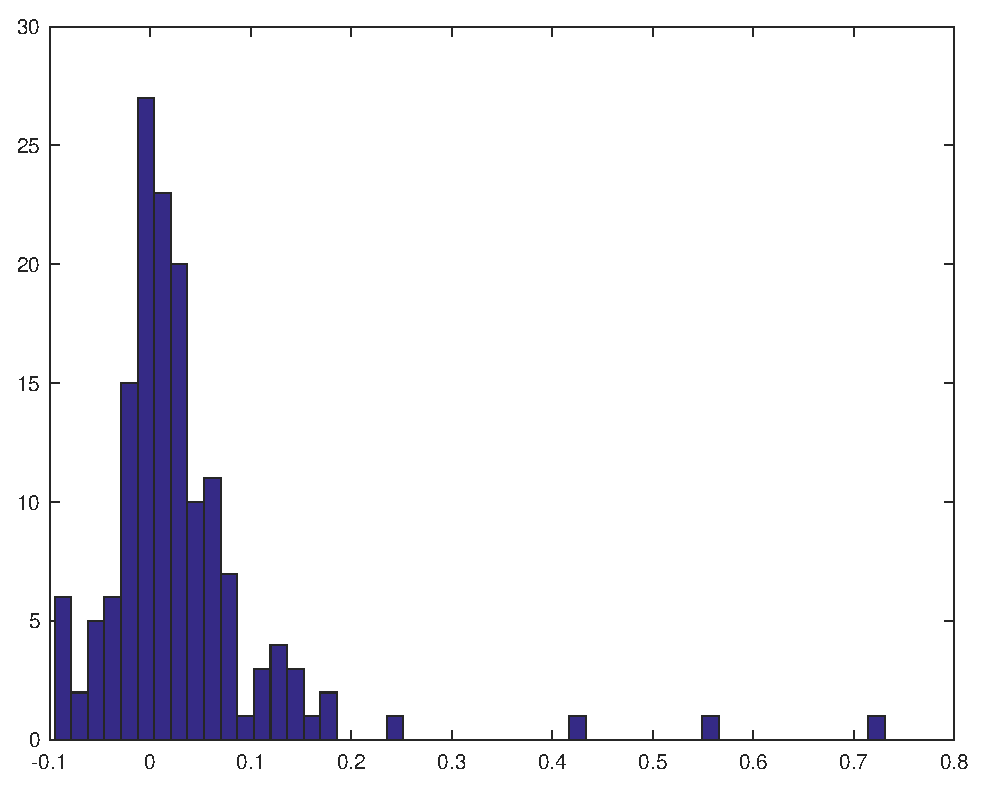
\includegraphics [width=4in]{lab1_04.eps}


\subsection*{the gradient algorithm}



\subsection*{istogrammi}


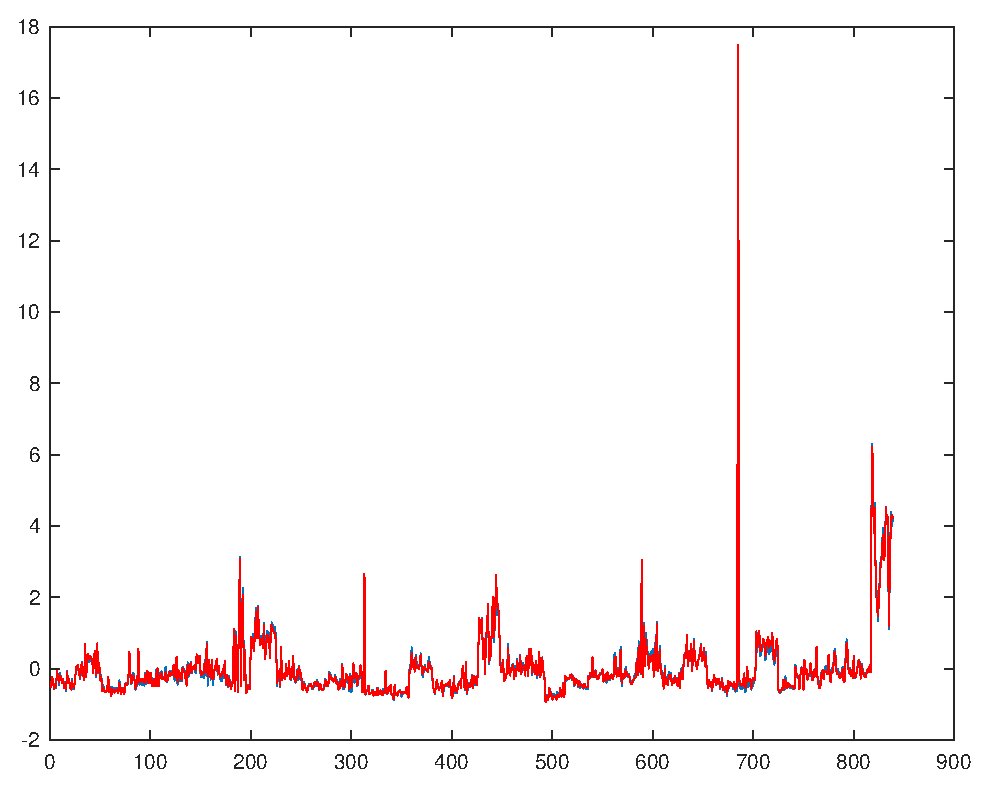
\includegraphics [width=4in]{lab1_05.eps}

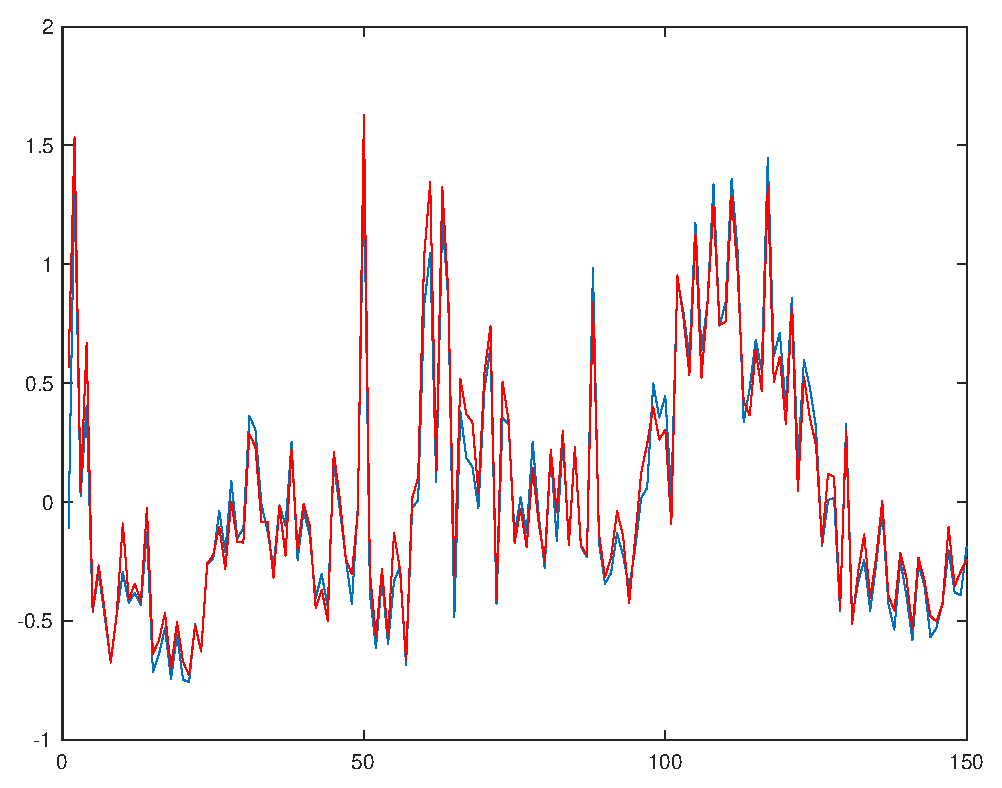
\includegraphics [width=4in]{lab1_06.eps}

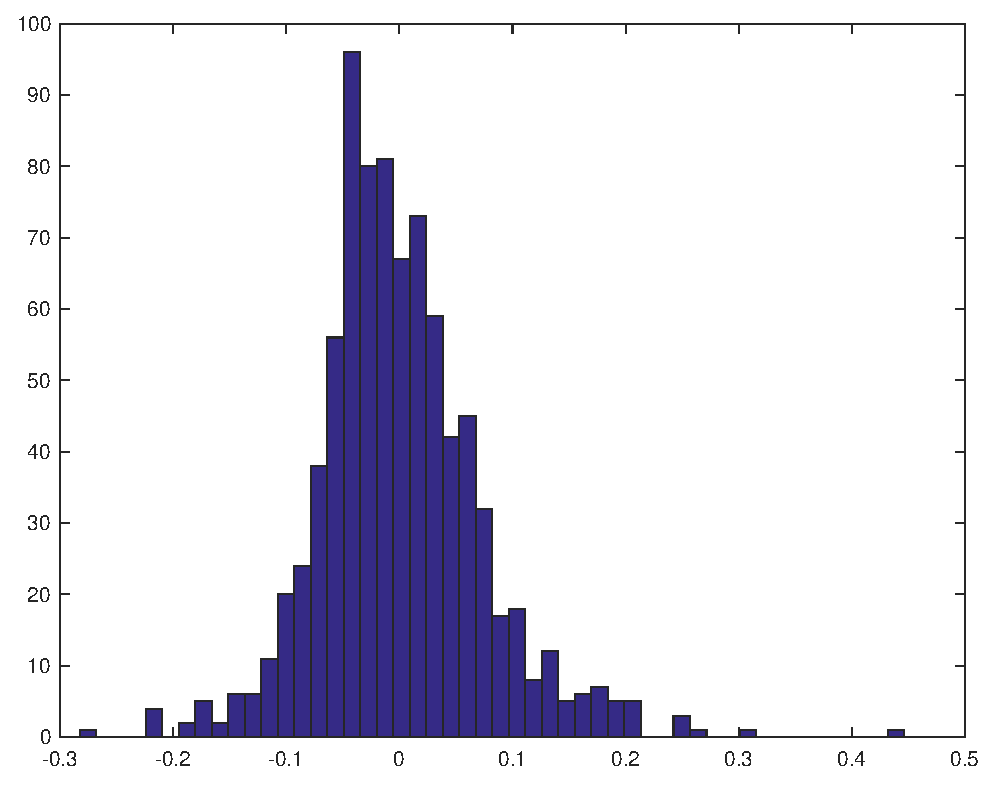
\includegraphics [width=4in]{lab1_07.eps}

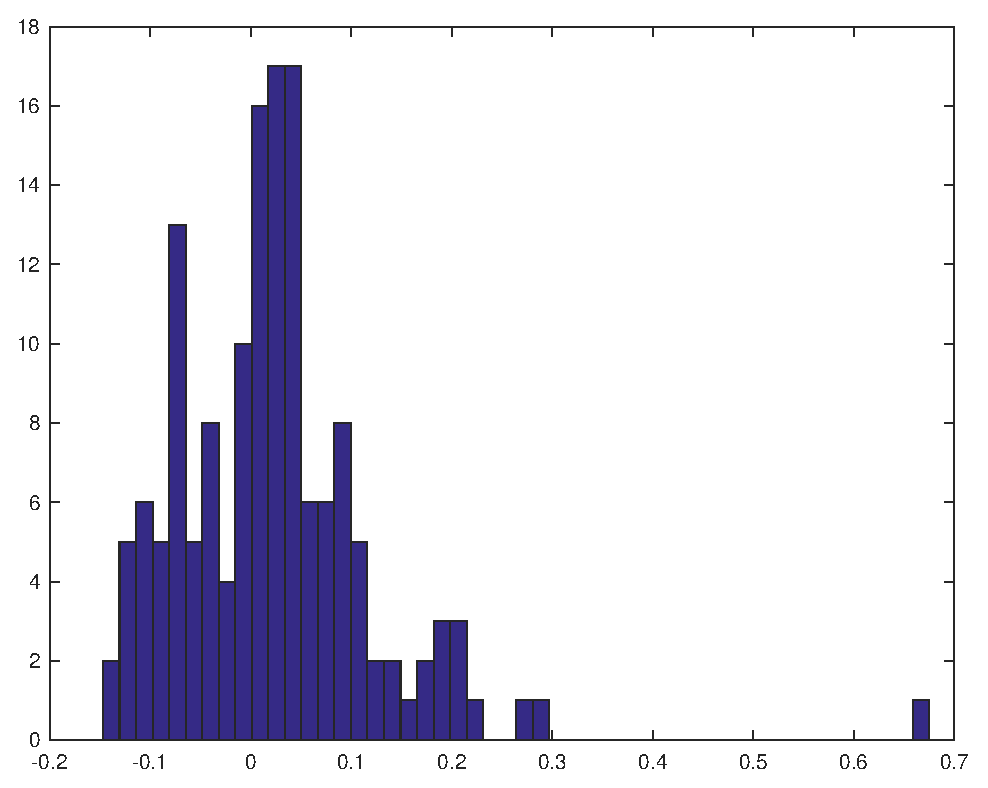
\includegraphics [width=4in]{lab1_08.eps}


\subsection*{steepest descent}



\subsection*{istogrammi}


\includegraphics [width=4in]{lab1_09.eps}

\includegraphics [width=4in]{lab1_10.eps}

\includegraphics [width=4in]{lab1_11.eps}

\includegraphics [width=4in]{lab1_12.eps}



\end{document}
    
